% Generated by jats2tex@0.11.1.0
\documentclass{article}
\usepackage{scielo}

\newcommand{\journalid}{Bull World Health Organ}
\newcommand{\journaltitle}{Bulletin of the World Health Organization}
\newcommand{\abbrevjournaltitle}{Bull. World Health Organ.}
\newcommand{\issnppub}{0042-9686}
\newcommand{\publishername}{World Health Organization}
\newcommand\articleid{\textsc{blt}.13.118810}
\newcommand\articledoi{\textsc{doi} 10.2471/\textsc{blt}.13.118810}
\def\subject{Round table}
\title{Tackling health workforce challenges to universal health coverage:
setting targets
and measuring progress\titlegroup{}}
\newcommand{\transtitlefr}{Relever les défis des effectifs de santé pour
réaliser la couverture sanitaire universelle: établir les objectifs et mesurer
les
progrès}
\newcommand{\transtitlees}{Abordar los desafíos del personal sanitario para
alcanzar la cobertura
universal de la salud: fijación de objetivos y evaluación del progreso}
\newcommand{\alttitleauthor}{Giorgio Cometto \& Sophie Witter}
\newcommand{\alttitle}{Tackling workforce challenges to achieve
\textsc{uhc}}
\author[{a}]{Cometto, Giorgio}
\author[{b}]{Witter, Sophie}
\affil[a]{World Health Organization}
\affil[b]{Queen Margaret University}
\def\authornotes{Correspondence to Giorgio Cometto (\mbox{e-mail}:
giorgiocometto@hotmail.com).}
\date{ 11 2013}
\def\volume{91}
\def\issue{11}
\def\fpage{881}
\def\lpage{885}
\newcommand{\cclicense}{(c) World Health Organization (\textsc{who}) 2013. All rights
reserved. $^{\tiny{\textregistered}}$ }
\newcommand{\copyrightyear}{2013}
%%% Nota %%%%%%%%%%%%%%%%%%%%%%%%%%%%%%%%%%%%%%%%%%%%%%%%%%%%%%%%
\expandafter\newcommand\csname \endcsname{
None declared.}

\begin{document}
\selectlanguage{english}
\newcommand{\lingua}{Inglês}
\maketitle
\tableofcontents

\begingroup
\renewcommand{\section}[1]{\subsection*{#1}}

\begin{abstract}

Human resources for health (\textsc{hrh}) will have to be strengthened if universal
health coverage (\textsc{uhc})
is to be achieved. Existing health workforce benchmarks focus exclusively on the
density of
physicians, nurses and midwives and were developed with the objective of
attaining relatively high
coverage of skilled birth attendance and other essential health services of
relevance to the health
Millennium Development Goals (\textsc{mdg}s). However, the attainment of \textsc{uhc} will depend
not only on the
availability of adequate numbers of health workers, but also on the
distribution, quality and
performance of the available health workforce. In addition, as noncommunicable
diseases grow in
relative importance, the inputs required from health workers are changing. New,
broader
health-workforce benchmarks – and a corresponding monitoring framework –
therefore
need to be developed and included in the agenda for \textsc{uhc} to catalyse attention
and investment in this
critical area of health systems. The new benchmarks need to reflect the more
diverse composition of
the health workforce and the participation of community health workers and
mid-level health workers,
and they must capture the multifaceted nature and complexities of \textsc{hrh}
development, including equity
in accessibility, sex composition and quality.

\ifdef{\kwdgroup}{\iflanguage{portuges}{\medskip\noindent\textbf{Palavras-chave:} \kwdgroup}{}}{}
\ifdef{\kwdgroupen}{\iflanguage{english}{\medskip\noindent\textbf{Keywords:}
\kwdgroupen}{}}{}
\ifdef{\kwdgroupes}{\iflanguage{spanish}{\medskip\noindent\textbf{Palavras
claves:} \kwdgroupes}{}}{}
\ifdef{\kwdgroupfr}{\iflanguage{french}{\medskip\noindent\textbf{Mots clés:}
\kwdgroupfr}{}}{}
\end{abstract}
\endgroup

\begingroup
\renewcommand{\section}[1]{\subsection*{#1}}
\begin{otherlanguage}{french}
\renewcommand{\abstractname}{Résumé}
\begin{abstract}

Les ressources humaines de la santé devront être renforcées pour pouvoir
réaliser la couverture sanitaire universelle. Les points de référence existants
des effectifs de santé se concentrent exclusivement sur la densité des
médecins, infirmiers et sages-femmes, et ils ont été développés
avec l'objectif d'atteindre une couverture relativement élevée des accouchements
médicalisés et des autres services de santé essentiels qui sont importants pour
la réalisation des objectifs du Millénaire pour le développement (\textsc{omd}) de la
santé. Cependant, la réalisation de la couverture sanitaire universelle ne
dépendra pas seulement de la disponibilité d'un nombre approprié de
professionnels de la santé, mais également de la distribution, de la qualité et
de la performance des effectifs de santé disponibles. En outre, comme le nombre
des maladies
non transmissibles ne cesse de croître, les contributions requises de la part
des
professionnels de la santé sont en train de changer. Des points de référence
nouveaux et plus larges des effectifs de santé – et un cadre de suivi
correspondant
– doivent donc être développés et inclus dans l'agenda pour la
couverture sanitaire universelle afin de catalyser l'attention et les
investissements dans ce
domaine critique des systèmes de santé. Les nouveaux points de référence
doivent refléter la composition plus diverse des effectifs de santé et la
participation des agents sanitaires des collectivités et des agents sanitaires
de niveau
intermédiaire, et ils doivent saisir la nature polymorphe et la complexité du
développement des ressources humaines de la santé, y compris en ce qui concerne
l'équité dans l'accessibilité, la composition sexospécifique et la
qualité.

\ifdef{\kwdgroupfr}{\medskip\noindent\textbf{Mots clés:} \kwdgroupfr}{}
\end{abstract}
\end{otherlanguage}
\endgroup

\begingroup
\renewcommand{\section}[1]{\subsection*{#1}}
\begin{otherlanguage}{spanish}
\renewcommand{\abstractname}{Resumen}
\begin{abstract}

Es fundamental fortalecer la acción de los recursos humanos en sanidad (\textsc{rhs})
para alcanzar
la cobertura universal de la salud (\textsc{cus}). Los parámetros de referencia actuales
sobre el
personal sanitario se centran exclusivamente en la densidad de médicos,
enfermeros y
comadronas, y se desarrollaron con el fin de alcanzar una cobertura
relativamente alta de asistencia
especializada durante el parto y otros servicios de salud esenciales, que fueran
para lograr los
Objetivos de Desarrollo del Milenio (\textsc{odm}). Sin embargo, la consecución de la
cobertura
universal de la salud no solo depende de la disponibilidad de un número adecuado
de personal
sanitario, sino también de la distribución, la calidad y el desempeño del
personal sanitario disponible. Además, la contribución necesaria por parte del
personal sanitario cambia a medida que la importancia de las enfermedades no
transmisibles crece
relativamente. Por lo tanto, es necesario desarrollar e incluir en el programa
otros
parámetros de referencia más amplios y actuales, así como su marco de
seguimiento
correspondiente, de modo que los trabajadores comunitarios de salud puedan
catalizar la
atención y la inversión en esta área clave del sistema sanitario. Los nuevos
puntos de referencia deben reflejar la composición más plural del personal
sanitario y
la participación de los trabajadores comunitarios de salud, así como de los
trabajadores
sanitarios de nivel medio. De esta manera, deben captar las múltiples facetas y
complejidades
del desarrollo de los recursos humanos para sanidad, incluyendo la equidad en la
accesibilidad, la
composición por sexo y la calidad.

\ifdef{\kwdgroupes}{\medskip\noindent\textbf{Palavras claves:} \kwdgroupes}{}
\end{abstract}
\end{otherlanguage}
\endgroup

\begingroup
\renewcommand{\section}[1]{\subsection*{#1}}
\begin{otherlanguage}{russian}
\renewcommand{\abstractname}{Резюме}
\begin{abstract}

Для
достижения
всеобщего
охвата
медико-санитарной
помощью (ВОМСП),
необходимо
усилить
кадровые
ресурсы
здравоохранения
(КРЗ).
Существующие
в настоящее
время методы
оценки
достаточности
кадров
здравоохранения
сосредоточены
исключительно
на
обеспеченности
населения
врачами,
медсестрами и
акушерками и
были
разработаны с
целью
достигнуть
относительно
высоких
показателей
по количеству
профессиональных
акушеров и
других важных
медицинских
служб в
соответствии
с Целями
тысячелетия в
области
развития
здравоохранения.
Тем не менее,
достижение
всеобщего
охвата
зависит не
только от
адекватного
количества
работников
здравоохранения,
но также от
распределения,
качества и
профессиональных
показателей
доступных
кадровых
ресурсов
здравоохранения.
Кроме того, с
ростом
относительной
важности
лечения
неинфекционных
заболеваний
меняются
требования к
работникам
здравоохранения.
Поэтому
должны быть
разработаны и
включены в
программу
действий по
ВОМСП новые,
более широкие
методы оценки
кадровых
ресурсов
здравоохранения,
а также
соответствующая
система
наблюдения.
Это поможет
активизировать
привлечение
внимания и
инвестиций к
этой
исключительно
важной
области
системы
здравоохранения.
Новые методы
оценки должны
отражать
многообразный
состав
кадровых
ресурсов
здравоохранения
и
задействование
местных
медработников,
а также
работников
здравоохранения
среднего
звена. Кроме
того, эти
оценки должны
отражать
многопрофильность
и сложность
развития КРЗ,
включая
равенство при
обеспечении
доступности,
половой
состав и
качество
подготовки.

\end{abstract}
\ifdef{\kwdgroupru}{\medskip\noindent\textbf{ключевые слова:} \kwdgroupru}{}
\end{otherlanguage}
\endgroup
\section{Introduction}

The eight Millennium Development Goals
(\textsc{mdg}s)\textsuperscript{[}\textsuperscript{1}\textsuperscript{]}

have been credited with catalysing a greater focus on the development priorities
they targeted
– poverty reduction, gender equality, primary education, maternal and child
health, control
of major diseases, environmental issues, and partnerships for development – and
with
mobilizing the relevant resources. With three of the \textsc{mdg}s being health-related,
health is awarded a
high priority in the current framework. The progress being made towards
achieving these three goals
is inequitable within and across countries, but despite this, many countries are
recording
improvements in health outcomes.\textsuperscript{[}\textsuperscript{2}\textsuperscript{]}

However, limitations in the \textsc{mdg} framework – and particularly in the
health-related \textsc{mdg}s
– are being recognized: a lack of attention to
equity,\textsuperscript{[}\textsuperscript{3}\textsuperscript{]}
the neglect of health issues that were not explicitly included in any of the
\textsc{mdg}s, and the fragmentation of efforts targeted at the different health
priorities (the latter might
have contributed to a narrowly selective focus on development assistance for
health).\textsuperscript{[}\textsuperscript{4}\textsuperscript{]}
The targets and indicators currently used for the
health-related \textsc{mdg}s focus on increasing the coverage of some priority health
services – such
as skilled birth attendance – and on improving health outcomes in relation to
maternal
health, child health and infectious diseases. However, none of the \textsc{mdg} targets
refers explicitly to
the health system actions required to attain such objectives. Yet it has been
evident for over a
decade that only by overcoming the structural deficiencies of health systems –
including
those related to governance, the health workforce, information systems, health
financing and supply
chains – will it be possible to improve specific outcomes for individual
diseases or
population subgroups.\textsuperscript{[}\textsuperscript{5}\textsuperscript{]}

Although econometric analyses have confirmed that an adequate health workforce
is necessary for
the delivery of essential health services and improvement in health
outcomes,\textsuperscript{[}\textsuperscript{6}\textsuperscript{]}\textsuperscript{,}\textsuperscript{[}\textsuperscript{7}\textsuperscript{]}
there
have been systemic failures in the planning, forecasting, development and
management of human
resources for health (\textsc{hrh}).\textsuperscript{[}\textsuperscript{8}\textsuperscript{]}\textsuperscript{,}\textsuperscript{[}\textsuperscript{9}\textsuperscript{]}
This has led to unacceptable variations in the
availability, distribution, capacity and performance of health workers, and
these have resulted, in
turn, in uneven quality and coverage of health services. In many low-income
countries, acute
shortages in the health workforce have been compounded by the emigration of
health workers to
high-income countries that offer better working conditions. The situation has
heightened a sense of
injustice that culminated in the adoption, in 2010, of the \textsc{who} Global Code of
Practice on the
International Recruitment of Health
Personnel.\textsuperscript{[}\textsuperscript{10}\textsuperscript{]}

\section{Health workforce benchmarks}

\textit{The world health report 2006}
included an estimate of the minimum density
threshold of physicians, nurses and midwives deemed generally necessary to
attain a high coverage of
skilled birth attendance: 2.28 per 1000
population.\textsuperscript{[}\textsuperscript{9}\textsuperscript{]}
According to the statistics available when the report was published, 57
countries fell below this benchmark and an additional 4.3 million health workers
would be required
to achieve the minimum density globally.

Thanks to its grounding in evidence, its relative simplicity and the fact that
it could be easily
standardized, the minimum density of physicians, nurses or midwives suggested in
\textit{The world
health report 2006}
– 2.28 per 1000 population – has become the most widely
used health workforce “target”. It was adopted in the commitments of the Group
of
Eight (G8) in 2008\textsuperscript{[}\textsuperscript{11}\textsuperscript{]}
and has served as a basis for
several monitoring and accountability processes that were either focused on the
health
workforce\textsuperscript{[}\textsuperscript{12}\textsuperscript{]}
or had a different and broader
focus.\textsuperscript{[}\textsuperscript{13}\textsuperscript{]}
However, this benchmark focuses
exclusively on physicians, nurses and midwives and was developed with the
objective of attaining
relatively high coverage of selected essential health services of relevance to
the health \textsc{mdg}s. In
today's world, it is no longer adequate in the health workforce discourse for at
least four
reasons:

The evidence underpinning the threshold value was based on data on immunization
coverage and
skilled birth attendance. No consideration was given to health workforce
requirements with respect
to a wider range of health services, including the control and treatment of
noncommunicable
diseases.

The benchmark only allows the identification of inadequacies in the numbers of
health workers. In
the attainment of universal health coverage (\textsc{uhc}), many other challenges of
equal – if not
greater – importance exist, such as issues relating to access to, and the
quality and
performance of, the health workforce that were not captured by the simple
density-based benchmark.
Aspects such as distribution, responsiveness, affordability and productivity
were crucially
missing.

The macroeconomic implications of attaining the density benchmark have not been
examined. It has
been estimated that some low-income countries would have to allocate 50\% of
their gross domestic
product to health to be able to reach the
benchmark.\textsuperscript{[}\textsuperscript{14}\textsuperscript{]}

The benchmark only relates to physicians, nurses and midwives. However,
community health
workers\textsuperscript{[}\textsuperscript{15}\textsuperscript{]}\textsuperscript{,}\textsuperscript{[}\textsuperscript{16}\textsuperscript{]}
and mid-level health workers\textsuperscript{[}\textsuperscript{17}\textsuperscript{]}
can also improve the availability and accessibility of health services while
maintaining – when appropriately trained and managed – quality standards that
are
similar to those of cadres undergoing longer training. Despite a growing
evidence base and a
significant political momentum in support of their role, including through the
global One Million
Community Health Workers Campaign and similar
initiatives,\textsuperscript{[}\textsuperscript{18}\textsuperscript{]}\textsuperscript{,}\textsuperscript{[}\textsuperscript{19}\textsuperscript{]}
these cadres
are often operating at the margins of health systems and are largely excluded
from \textsc{hrh} information
systems and benchmarks.

A few other benchmarks have been used, such as the Sphere
standards.\textsuperscript{[}\textsuperscript{20}\textsuperscript{]}
However, these benchmarks – which call for at least one
physician and 50 community health workers for every 50 000 population – are only
of
primary relevance to humanitarian operations in refugee settings.

\begin{enumerate}[i.]
\item
The evidence underpinning the threshold value was based on data on immunization
coverage and
skilled birth attendance. No consideration was given to health workforce
requirements with respect
to a wider range of health services, including the control and treatment of
noncommunicable
diseases.

\item
The benchmark only allows the identification of inadequacies in the numbers of
health workers. In
the attainment of universal health coverage (\textsc{uhc}), many other challenges of
equal – if not
greater – importance exist, such as issues relating to access to, and the
quality and
performance of, the health workforce that were not captured by the simple
density-based benchmark.
Aspects such as distribution, responsiveness, affordability and productivity
were crucially
missing.

\item
The macroeconomic implications of attaining the density benchmark have not been
examined. It has
been estimated that some low-income countries would have to allocate 50\% of
their gross domestic
product to health to be able to reach the
benchmark.\textsuperscript{[}\textsuperscript{14}\textsuperscript{]}

\item
The benchmark only relates to physicians, nurses and midwives. However,
community health
workers\textsuperscript{[}\textsuperscript{15}\textsuperscript{]}\textsuperscript{,}\textsuperscript{[}\textsuperscript{16}\textsuperscript{]}
and mid-level health workers\textsuperscript{[}\textsuperscript{17}\textsuperscript{]}
can also improve the availability and accessibility of health services while
maintaining – when appropriately trained and managed – quality standards that
are
similar to those of cadres undergoing longer training. Despite a growing
evidence base and a
significant political momentum in support of their role, including through the
global One Million
Community Health Workers Campaign and similar
initiatives,\textsuperscript{[}\textsuperscript{18}\textsuperscript{]}\textsuperscript{,}\textsuperscript{[}\textsuperscript{19}\textsuperscript{]}
these cadres
are often operating at the margins of health systems and are largely excluded
from \textsc{hrh} information
systems and benchmarks.

\end{enumerate}

\section{Evolving health workforce needs}

The renewed focus on \textsc{uhc} in the health policy discourse – which culminated in
December
2012 in the adoption of a United Nations General Assembly resolution on global
health and foreign
policy – has contributed to a wider recognition of the need for an “adequate
skilled,
well-trained and motivated [health]
workforce”.\textsuperscript{[}\textsuperscript{21}\textsuperscript{]}

The progressive realization of the right to health for all people – and of \textsc{uhc} –
will entail a wide array of actions to address the specific needs of each
country. As national
health systems in low- and middle-income countries try to broaden the services
they provide to cover
noncommunicable diseases as well, new demands will be made on their health
workers. Population
demands for more equitable access to health care of good quality will also have
to be reflected in
efforts at securing greater accessibility of health workers – especially in
rural and other
underserved areas\textsuperscript{[}\textsuperscript{22}\textsuperscript{]}
– and improving their
competence and performance. There will also be an increasing demand for greater
efficiency: in
general, the countries that are facing the greatest obstacles to the attainment
of \textsc{uhc} are also the
most fiscally constrained. Affordable approaches to boost the performance of
health workers are
urgently required. There may be trade-offs between the broader \textsc{hrh} needs
entailed in the \textsc{uhc}
paradigm and the financial constraints faced by many countries. It may be
possible to increase the
cost-effectiveness of an expanding health system by awarding more prominent
roles to community
health workers and mid-level health workers. Similarly, the adoption of
appropriate management
systems and incentive structures could help to optimize the performance of
existing health workers
and reduce wasteful spending.\textsuperscript{[}\textsuperscript{23}\textsuperscript{]}

Guaranteeing \textsc{uhc} is a multifaceted endeavour. To approach the issue through the
health workforce
lens, it is necessary to go beyond mere numbers and address gaps in equitable
distribution,
competency, quality, motivation, productivity and performance. Improving access
to effective
coverage will not be possible otherwise (Fig.~\ref{fig:F1}
).

Human resources for health actions required to achieve universal health coverage

Source: Jim Campbell and Giorgio Cometto (2012), adapted from Tanahashi (1978).

On the path towards \textsc{uhc}, fundamental changes will have to be adopted by
countries and by the
global health community in relation to how health workers are trained, deployed,
managed and
supported.\textsuperscript{[}\textsuperscript{24}\textsuperscript{]}
The role of the public sector in
shaping health labour market forces will also have to be strengthened. A
critical element in this
endeavour is the inclusion of \textsc{hrh} benchmarks and of a corresponding monitoring
framework in the \textsc{uhc}
agenda.

\begin{figure}
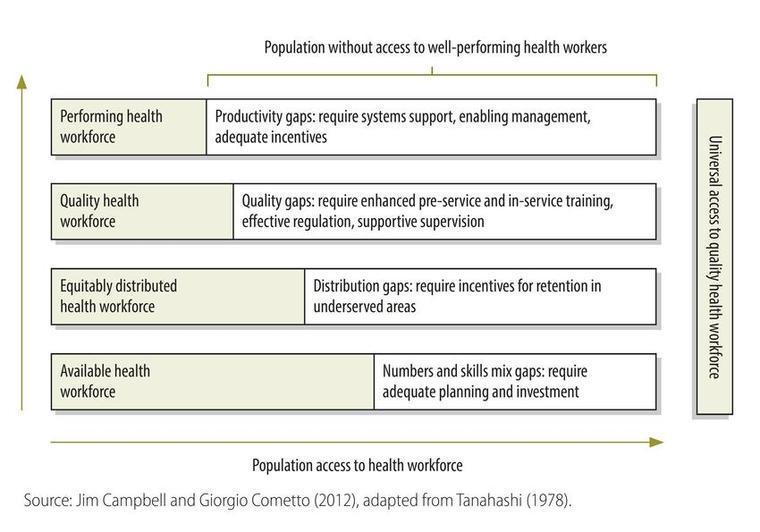
\includegraphics[width=\textwidth]{0042-9686-bwho-91-11-881-F1}
\caption{}\label{fig:F1}
\end{figure}

\section{Aiming for universal health coverage}

\textsc{hrh} are not an end in themselves but the indispensable means to achieving
improved health
outcomes. Aware of the importance of measurable targets and linked
accountability mechanisms in
stimulating action, countries and the international community should include a
health-workforce-specific benchmark in the framework for \textsc{uhc} and the post-2015
development agenda.
The inclusion of \textsc{hrh} benchmarks in the post-2015 agenda could help to foster
collaboration between
countries and global partners and to focus policy actions and investments where
they are most
required.

The development of new benchmarks in the field of \textsc{hrh} should take into account
several
interrelated factors, including:

population growth and the demographic transition;

the growing burden of noncommunicable diseases and the corresponding changes in
demand for health
services by citizens;

the need to adapt the skills and competencies of health workers to match these
changed
demands;

an appreciation of health workforce challenges other than numerical shortages,
and of the
potential contributions of cadres other than physicians, nurses and midwives in
improving health
service availability and accessibility – especially in those disrupted health
systems that
face the most acute challenges;

the role of non-state actors, which has never been adequately captured in
previous benchmarks or
in the corresponding monitoring frameworks.

New benchmarks are required that give a better reflection of the diverse
composition of the
health workforce. They should take account of the contributions that are made by
social workers who
are involved in long-term care and by community health workers and mid-level
health workers. The
inclusion of these other cadres could result in targets that are realistically
attainable even by
low-income countries. Recent costing studies suggest that providing care through
community health
workers is affordable.\textsuperscript{[}\textsuperscript{25}\textsuperscript{]}
However, any additions to
the roles and expectations of health workers are likely to increase resource
requirements.

Even adopting a more affordable skills mix and increasing efficiency in \textsc{hrh}
spending through a
renewed emphasis on performance and quality of care, the financial path towards
\textsc{uhc} for some
low-income countries and fragile states will inevitably involve, at least in the
short-term, a role
for official development assistance. Feng Zhao et al. discuss in an editorial in
this theme issue
how to maximize the returns of external financing for
\textsc{hrh}.\textsuperscript{[}\textsuperscript{26}\textsuperscript{]}

\textsc{hrh} benchmarks should influence the planning, management, support and monitoring
of health
systems. They should also be reflected in the setting of the targets used – at
the national
and global level – to track progress towards \textsc{uhc} and the health priorities of
the post-2015
development agenda.

It would also be helpful, besides setting quantitative targets, to introduce an
equity lens and
explore needs in other dimensions, including the geographical distribution and
sex composition of
the health workforce. Minimum standards need to be established for all aspects
of health worker
performance – including responsiveness and competency and the associated
management,
financing and information systems. This round table base paper is complemented
by four
discussants,\textsuperscript{[}\textsuperscript{27}\textsuperscript{]}\textsuperscript{–}\textsuperscript{[}\textsuperscript{30}\textsuperscript{]}
on how to strike the right balance between benchmarks
that are sharp, actionable and measurable while simultaneously capturing the
multifaceted nature and
complexities of health workforce development.

\begin{enumerate}[i.]
\item
population growth and the demographic transition;

\item
the growing burden of noncommunicable diseases and the corresponding changes in
demand for health
services by citizens;

\item
the need to adapt the skills and competencies of health workers to match these
changed
demands;

\item
an appreciation of health workforce challenges other than numerical shortages,
and of the
potential contributions of cadres other than physicians, nurses and midwives in
improving health
service availability and accessibility – especially in those disrupted health
systems that
face the most acute challenges;

\item
the role of non-state actors, which has never been adequately captured in
previous benchmarks or
in the corresponding monitoring frameworks.

\end{enumerate}

\section*{References}
\begin{itemize}

\item[1] Waage J, Banerji R, Campbell O, Chirwa E, Collender G, Dieltiens V et
al. The
Millennium Development Goals: a cross-sectoral analysis and principles for goal
setting after 2015:
Lancet and London International Development Centre Commission. Lancet
2010;376:991–1023. doi:
http://dx.doi.org/10.1016/S0140-6736(10)61196-8 \textsc{pmid}:20833426

\item[2] United Nations Regional Information Centre for Western Europe
[Internet]. UN \textsc{mdg}
report, 2012, stresses need for a true global partnership. Brussels: \textsc{unricwe};
2012. Available from:
http://www.unric.org/en/latest-un-buzz/27661-un-mdg-report-2012-stresses-need-fo
r-a-true-global-partnership
[accessed 25 July 2013].

\item[3] Reidpath DD, Morel CM, Mecaskey JW, Allotey P. The Millennium
Development Goals fail
poor children: the case for equity-adjusted measures. \textit{PLoS Med}
2009;6:e1000062.
doi: http://dx.doi.org/10.1371/journal.pmed.1000062 \textsc{pmid}:19399155

\item[4] Samb B, Evans T, Dybul M, Atun R, Moatti JP, Nishtar S et al.; World
Health
Organization Maximizing Positive Synergies Collaborative Group. An assessment of
interactions
between global health initiatives and country health systems. \textit{Lancet}

2009;373:2137–69. doi: http://dx.doi.org/10.1016/S0140-6736(09)60919-3
\textsc{pmid}:19541040

\item[5] Travis P, Bennett S, Haines A, Pang T, Bhutta Z, Hyder AA et al.
Overcoming
health-systems constraints to achieve the Millennium Development Goals.
\textit{Lancet}

2004;364:900–6. doi: http://dx.doi.org/10.1016/S0140-6736(04)16987-0
\textsc{pmid}:15351199

\item[6] Anand S, Bärnighausen T. Health workers and vaccination coverage in
developing
countries: an econometric analysis. \textit{Lancet}
2007;369:1277–85. doi:
http://dx.doi.org/10.1016/S0140-6736(07)60599-6 \textsc{pmid}:17434403

\item[7] Anand S, Bärnighausen T. Human resources and health outcomes:
cross-country
econometric study. \textit{Lancet}
2004;364:1603–9. doi:
http://dx.doi.org/10.1016/S0140-6736(04)17313-3 \textsc{pmid}:15519630

\item[8] \textit{Human resources for health – overcoming the crisis}. Cambridge:
Joint Learning Initiative; 2004. Available from:
www.who.int/hrh/documents/JLi\_{}hrh\_{}report.pdf
[accessed 25 July 2013].

\item[9] \textit{The world health report 2006 – working together for health}. Geneva:
\textsc{who}; 2006. Available from: http://www.who.int/whr/2006 [accessed 25 July 2013].

\item[10] Resolution \textsc{wha}63.16. \textsc{who} Global Code of Practice on the International
Recruitment of
Health Personnel. In: \textit{Sixty-third World Health Assembly, Geneva, 21 May
2010. Resolutions
and decisions}. Geneva: World Health Organization; 2010. Available from:
http://apps.who.int/gb/ebwha/pdf\_{}files/\textsc{wha}63/A63\_{}R16-en.pdf [accessed 25
July
2013].

\item[11] \textit{G8 Hokkaido Toyako Summit Leaders Declaration}. Toyako: Group of
Eight; 2008. Available from:
http://www.mofa.go.jp/policy/economy/summit/2008/doc/doc080714\_{}\_{}en.html
[accessed 25 July 2013].

\item[12] Global Health Workforce Alliance [Internet]. Reviewing progress,
renewing
commitment: launch of the progress report on the Kampala Declaration and Agenda
for Global Action.
Geneva: World Health Organization; 2011. Available from:
http://www.who.int/workforcealliance/forum/2011/progressreportlaunch [accessed
25 July
2013].

\item[13] \textit{Building a future for women and children: the 2012 report}. Geneva:
World Health Organization; 2012. Available from:
http://www.countdown2015mnch.org/reports-and-articles/2012-report [accessed 25
July
2013].

\item[14] Bossert TJ, Ono T. Finding affordable health workforce targets in
low-income
nations. \textit{Health Aff (Millwood)}
2010;29:1376–82. doi:
http://dx.doi.org/10.1377/hlthaff.2009.0443 \textsc{pmid}:20606191

\item[15] Lewin S, Munabi-Babigumira S, Glenton C, Daniels K, Bosch-Capblanch X,
van Wyk BE et
al. Lay health workers in primary and community health care for maternal and
child health and the
management of infectious diseases. \textit{Cochrane Database Syst Rev}
2010;3:CD004015.
\textsc{pmid}:20238326

\item[16] Global Health Workforce Alliance [Internet]. Community health workers.
Geneva: \textsc{ghwa};
2010. Available from:
http://www.who.int/workforcealliance/knowledge/themes/community [accessed 25
July 2013].

\item[17] Lassi ZS, Cometto G, Huicho L, Bhutta ZA. Quality of care provided by
mid-level
health workers: systematic review and meta-analysis. \textit{Bull World Health
Organ}

2013;91:824–33.

\item[18] One million community health workers [Internet]. Grant to help
coordinate campaign
to train one million community health workers in sub-Saharan Africa. New York:
One Million Community
Health Workers Campaign; 2013. Available from:
http://www.1millionhealthworkers.org [accessed 25
July 2013].

\item[19] Singh P, Sachs JD. 1 million community health workers in sub-Saharan
Africa by 2015.
\textit{Lancet}
2013;382:363–5. doi: http://dx.doi.org/10.1016/S0140-6736(12)62002-9
\textsc{pmid}:23541538

\item[20] \textit{Humanitarian charter and minimum standards in humanitarian
response}. Geneva: The Sphere Project; 2011. Available from:
http://www.sphereproject.org/resources/download-publications/?search=1\&keywords
=\&language=English\&category=22
[accessed 25 July 2013].

\item[21] Resolution A. 67/L.36. Resolution on global health and foreign policy.
In:
\textit{Sixty-seventh session of the United Nations General Assembly, New York,
6 December
2012}. New York: United Nations; 2012. Available from:
http://www.un.org/ga/search/view\_{}doc.asp?symbol=A/67/L.36 [accessed 25 July
2013].

\item[22] Dolea C, Stormont L, Braichet JM. Evaluated strategies to increase
attraction and
retention of health workers in remote and rural areas. \textit{Bull World Health
Organ}

2010;88:379–85. doi: http://dx.doi.org/10.2471/\textsc{blt}.09.070607 \textsc{pmid}:20461133

\item[23] \textit{The world health report 2010 – health systems financing: the
path to
universal coverage}. Geneva: World Health Organization; 2010. Available from:
http://www.who.int/whr/2010 [accessed 25 July 2013].

\item[24] Bhutta ZA, Chen L, Cohen J, Crisp N, Evans T, Fineberg H et al.
Education of health
professionals for the 21st century: a global independent commission.
\textit{Lancet}

2010;375:1137–8. doi: http://dx.doi.org/10.1016/S0140-6736(10)60450-3
\textsc{pmid}:20362799

\item[25] McCord GC, Liu A, Singh P. Deployment of community health workers
across rural
sub-Saharan Africa: financial considerations and operational assumptions.
\textit{Bull World Health
Organ}
2013;91:244–53B. doi: http://dx.doi.org/10.2471/\textsc{blt}.12.109660
\textsc{pmid}:23599547

\item[26] Zhao F, Squires N, Weakliam D, Van Lerberghe W, Soucat A, Toure K et
al. Investing
in human resources for health: the need for a paradigm shift for the global
health community over
the next decade. \textit{Bull World Health Organ}
2013;91:799–9A.

\item[27] Boerma T, Siyam A. Health workforce indicators: let’s get real.
\textit{Bull World
Health Organ}
2013;91:886.

\item[28] Campbell J. Towards universal health coverage: a health workforce fit
for purpose
and practice. \textit{Bull World Health Organ}
2013;91:886–7.

\item[29] Scheil-Adlung X. Health workforce benchmarks for universal health
coverage and
sustainable development. \textit{Bull World Health Organ}
2013;91:888.

\item[30] Baker BK. Empowering patients and strengthening communities for real
health
workforce and funding targets. \textit{Bull World Health Organ}

2013;91:889.

\end{itemize}

   \section*{Metadados não aplicados}
    \begin{itemize}
    \ifdef{\lingua}{\item[\textbf{língua do artigo}] \lingua}{}
    \ifdef{\journalid}{\item[\textbf{journalid}] \journalid}{}
    \ifdef{\journaltitle}{\item[\textbf{journaltitle}] \journaltitle}{}
    \ifdef{\journalsubtitle}{\item[\textbf{journalsubtitle}] \journalsubtitle}{}
    \ifdef{\historydateaccepted}{\item[\textbf{historydateaccepted}] \historydateaccepted}{}
    \ifdef{\historydatereceived}{\item[\textbf{historydatereceived}] \historydatereceived}{}
    \ifdef{\ack}{\item[\textbf{ack}] \ack}{}
    \ifdef{\transjournaltitle}{\item[\textbf{journaltitle}] \journaltitle}{}
    \ifdef{\transjournalsubtitle}{\item[\textbf{journalsubtitle}] \journaltitle}{}
    \ifdef{\abbrevjournaltitle}{\item[\textbf{abbrevjournaltitle}] \abbrevjournaltitle}{}
    \ifdef{\issnppub}{\item[\textbf{issnppub}] \issnppub}{}
    \ifdef{\issnepub}{\item[\textbf{issnepub}] \issnepub}{}
    \ifdef{\alttitleauthor}{\item[\textbf{alttitle}] \alttitleauthor}{}
    \ifdef{\alttitle}{\item[\textbf{alttitleauthor}] \alttitle}{}
    \ifdef{\publishername}{\item[\textbf{publishername}] \publishername}{}
    \ifdef{\publisherid}{\item[\textbf{publisherid}] \publisherid}{}
    \ifdef{\subject}{\item[\textbf{subject}] \subject}{} 
    \ifdef{\transtitle}{\item[\textbf{transtitle}] \transtitle}{}
    \ifdef{\authornotes}{\item[\textbf{authornotes}] \authornotes}{}
    \ifdef{\articleid}{\item[\textbf{articleid}] \articleid}{}
    \ifdef{\articledoi}{\item[\textbf{articledoi}] \articledoi}{}
    \ifdef{\volume}{\item[\textbf{volume}] \volume}{}
    \ifdef{\issue}{\item[\textbf{issue}] \issue}{}
    \ifdef{\fpage}{\item[\textbf{fpage}] \fpage}{}
    \ifdef{\lpage}{\item[\textbf{lpage}] \lpage}{}
    \ifdef{\permissions}{\item[\textbf{permissions}] \permissions}{}
    \ifdef{\copyrightyear}{\item[\textbf{copyrightyear}] \copyrightyear}{}

    \end{itemize}
\end{document}
